\documentclass[11pt,a4paper]{article}
\usepackage[czech]{babel}
\usepackage[utf8]{inputenc}
\usepackage{times}
\usepackage{url}
\usepackage[textwidth=15.2cm,textheight=23cm]{geometry}
\usepackage{xcolor}

\usepackage{graphicx}

%\usepackage{fancyvrb}
%\DefineVerbatimEnvironment{verbatim}{Verbatim}{}

\usepackage[bf]{caption}

\usepackage[hyperindex,
  plainpages=false,
  pdftex,
  colorlinks,
  pdfborder={0 0 0},
  pdfpagelabels]{hyperref}

\pdfcompresslevel=9

\newcommand{\myincludegraphics}[4]{
  \begin{figure}[!h]
  \centering
  \includegraphics[#1]{#2}
  \caption{#3.} \label{#4}
  \end{figure}
}

% titulní stránka a obsah
\newcommand{\titlepageandcontents}{
  \begin{titlepage}

\vspace*{1cm}

\begin{figure}[h]
  \centering
  
\includegraphics[height=6cm]{images/fit.pdf}
\end{figure}

\vspace*{20mm}

\begin{center}
\begin{huge}
Vysoké učení technické v Brně\\
Fakulta informačních technologií
\end{huge}
\end{center}

\vspace*{20mm}

\begin{center}
\begin{Huge}
\subject{} \\
\end{Huge}
\begin{huge}
Státnicové okruhy MSZ 2015\\
\end{huge}
\end{center}


\end{titlepage}


  \pagestyle{plain}
  \pagenumbering{roman}
  \setcounter{page}{1}
  %\tableofcontents

  \newpage
  \pagestyle{plain}
  \pagenumbering{arabic}
  \setcounter{page}{1}
}

\def\uv#1{\iflanguage{english}{``#1''}%
                              {\quotedblbase #1\textquotedblleft}}%

\newcommand\todo[1]{\textcolor{red}{[[TODO: #1]]}}
\newcommand\blindtextGray{\textcolor{gray}{\blindtext}}
\newcommand\comment[1]{}

\newcommand\subject[1]{Předmět}


% vim:set ft=tex expandtab enc=utf8:

\usepackage{amsmath}
\usepackage{moreverb}
\usepackage{float}


\renewcommand\subject[1]{PDS}

\begin{document} \sloppy
\titlepageandcontents

\section{Sítě Peer-to-Peer (P2P), Milgramův problém malého světa, model sítě P2P, směrování v P2P
sítích, strukturované a nestruktorvané sítě}
\subsection{Milgramův problém malého světa}\label{small_world}
\begin{itemize}
\item Základ pro P2P sítě.
\item Potřebuji předat informaci člověku, kterého znám (mám informace o tom, kde se narodil atp.), ale neznám jeho adresu. Jsem shopen mu zásilku předat, aniž bych ji posílal klasickou poštou, jenom skrze lidi, které on zná a já znám (známé mých znamých)? 
\item Tato otázka vychází z poznatku jaká je pravděpodobnost, že se znají dva náhodně vybraní lidé. A pokud se neznají osobně, tak přes kolik známých se znají.
\item V podstatě hledáme matematické struktury ve společnosti. Máme stovky tisíc bodů a ptáme se přes kolik mezilehlých bodů je možné vytvořit nejkratší cestu pro dva libovlné uzly.
\item Závěr zní, že jedinci, kteří používají \textbf{pouze lokální informace}, jsou \textbf{velmi efektivní} ve vytvoření nejkratší cesty mezi dvěma body v sociální síti. Z toho plyne, že propojení mezi dvěma jedinci v síti je možné pomocí malé posloupnosti známých.
\item Otázkou je, zda existuje decentralizovaný aloritmus, který najde řetězec mezi dvěma libovolnými body. Odpoveď je \textbf{ano, existuje}.
\end{itemize}
\subsubsection{Milgramův experiment}
\begin{itemize}
\item Úkolem bylo doručit dopis příteli v jiném státě.
\item Jako odesilatele vybral náhodných 160 lidí (předpoklad byl, že odesilateli byly zděleny informace o adresátovi -- jaké má povolání, kde studovat atp.).
\item Dopis bylo možné předávat jenom skrze známé.
\item Každý, kdo dostal zásilku, posílal potrzující dopis zpátky na Hradvard (výchozí bod).
\item Výsledkem bylo, že nejkratší řetěz zpráv vedl přes 2 lidi, nejdelší přes 11 a medián bylo 5 lidí. Závěr tedy je, že stačí 5 lidí.
\end{itemize}

\subsection{Peer--to--Peer sítě}
%---obrazek
\begin{figure}[h!]
\begin{center}
\scalebox{0.8}{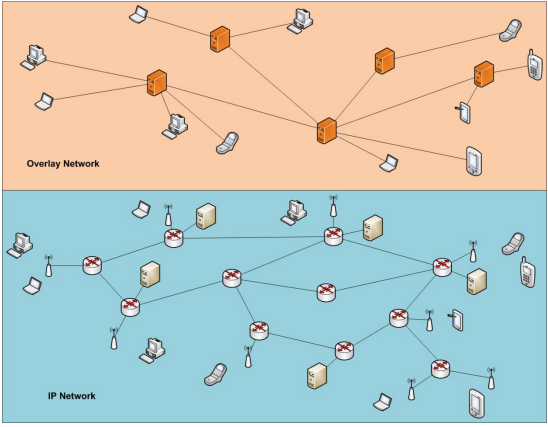
\includegraphics{images/overlay.png}}
\caption{Overlay u P2P sítí (oranžové).}
\label{p2p_overlay}
\end{center}
\end{figure}
%---konec obrazek
\begin{itemize}
\item P2P sítě jsou postavené nad IP, ale mají:
\begin{itemize}
\item Jinou koncepci architektury -- odlišná role uzlů.
\item Jiný způsob adresování -- adresování obsahem.
\item Jiný přístup ke směrování -- uzly se odpojují/připojují libovolně.
\item Jiné vlastnosti sítí -- samo--organizace, decentralismus.
\end{itemize}
\item Zdroje jsou dostupné všem -- slouží především pro sdílení zdrojů.
\item Základní operace v P2P sítích: připojení uzlu, odpojení uzlu a vyhledání objektu.
\item Všichni účastníci něco do sítě přinášejí a něco si z ní odnášejí (sdílím a stahuji).
\item Základem sítí P2P je \textbf{overlay} (vlastní nezávislá síť -- viz obrázek \ref{p2p_overlay}) -- síť, která je vybudovaná nad fyzickou architekturou (uzly z overlay se mapují na fyzické). Mezi uzly existuje komunikace a protokol -- řešeno speciálním SW.
\end{itemize}


\subsubsection{Typy P2P sítí}
\begin{itemize}
\item \textbf{Pravé P2P sítě} -- všechny uzly mají stejný význam (tj. pokud odeberu uzel ze sítě nemá to to vliv na ztrátu schopnosti sítě poskytovat dané služby).
\item \textbf{Hybridní P2P sítě} -- několik typů uzlů. Potřeba centrálního uzlu pro poskytování části nabízených služeb (tento bod slouží k autentizaci, indexování atp.). Jedná se o kombinaci P2P a klient--server.
\end{itemize}

\subsubsection{Vlastnosti sítí P2P}
\begin{itemize}
\item Samo--organizující se síť -- decentralizovaná topologie, uzly spolupracují na vytvoření a udržování sítě$\ldots$
\item Autonomní chování uzlů -- uzly se chovají dle vlastního nejlepšího rozhodnutí.
\item Rozšiřitelnost -- každý nový uzel přidává svou kapacitu systému.
\item Doba života uzlu --  doba životnosti uzlu je krátká a neodhadnutelná (parametr \uv{churn rate} -- odliv zákazníků).
\item Spolehlivost -- roste s redundancí uzlů a informací.
\end{itemize}

\subsection{Model P2P sítě}
%---obrazek
\begin{figure}[ht!]
\begin{center}
\scalebox{0.8}{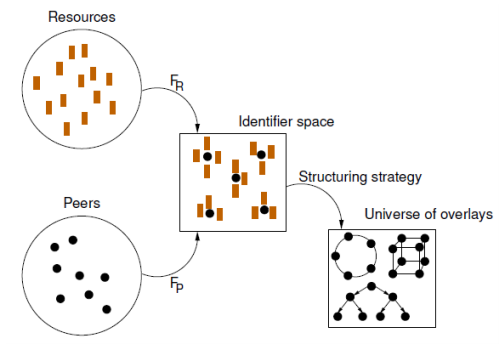
\includegraphics{images/model_p2p.png}}
\caption{Model P2P sítí.}
\label{p2p_model}
\end{center}
\end{figure}
%---konec obrazek
Model P2P sítě (viz obrázek \ref{p2p_model}) se skládá z komponent:
\begin{itemize}
\item Jmenný prostor $I$ -- prostor jmen, identifikuje uzly (dle hashe nějaké charakteristiky -- např. hash z IP, hash privátního klíče atp.) a zdroje (dle hashe názvu souboru, hashe názvu článku$\ldots$), které jsou tam připojené. \textbf{Musí obsahovat metriku blízkosti} (definice metriky viz MAT) kvůli vyhledávání atp.
\item Množina uzlů (peers) $P$
\item Množina zdrojů (resources) $R$ -- soubory, články$\ldots$
\item Mapování objektů $F_R : R \rightarrow I$ -- Přidělí zdrojům identifikátor z I.
\item Mapování uzlů $F_P : P \rightarrow I$ -- Přidělí uzlům jednoznačný identifikátor.
\item Struktura logické sítě -- vytváří vlastní síť z identifikačního prostoru.
\end{itemize}

\subsubsection{Struktura logické sítě overlay}
\begin{itemize}
\item Jedná se o orientovaný graf.
\item Operace připojení/odpojení uzlů.
\item Množina sousedů uzlu $p$ je dána \textbf{relací sousedství (neighborhood)} -- souvisí s vyhledáváním a říká, že pro každý uzel $p$ můžu mít množinu sousedních uzlů $N(p)$.
\item Důležitý parametr je \textbf{poloměr grafu} -- maximální vzdálenost mezi dvěma uzly grafu (menší poloměr -- rychlejší vyhledávání).
\end{itemize}

\subsubsection{Směrování}
\begin{itemize}
\item Směrování u všech druhů P2P sítí je na základě pouze \textbf{lokální} informace.
\item Směrování = předávání zprávy \textbf{route(p,m,i)} -- směrujeme zprávu $m$ na uzel $p$, který obsahuje objekt $i$.
\item Směrovací funkce = vybere v daném uzlu $p$ z množiny sousedů $N(p)$ takový uzel $q$, který je blíže (používá se metrika) k uzlu, který obsahuje objekt $i$.
\item Chybí globální synchronizace směrování -- mouhou nastat nekonzistence v lokální směrovací tabulce.
\end{itemize}

\subsubsection{Správa sítě P2P}
\begin{itemize}
\item Musí řešit dynamické připojování a odpojování uzlů -- proaktivní správa (neustále zasílám zprávy) či reaktivní mechanismy (pro speciální sítě).
\item Sledování aktuáně připojených sousedů.
\item Aktualizace směrovací tabulky.

\end{itemize}

\subsection{Nestrukturované sítě P2P}
\begin{itemize}
\item Využívají poznatky sociálních sítí a malého světa (viz kapitola \ref{small_world}).
\item Ukládání objektů nezávisí na propojení uzlů.
\item Neexistuje struktura uložení informace -- obsah (informace) je uložen v náhodně vybraném uzlu.
\item Uzel si může se svými sousedy vyměňovat zprávy -- např. dotaz na vyhledání konkrétní informace.
\item Nebezpečí vytvoření smyčky --  lze tomu zabránit např. použitím TTL (Time to live).
\item Neefektivní směrování.
\item Špatná lokalizace žřídka se vyskytujících objektů.
\item Směrování podle klíče (ID objektu) -- požadavek směrován do uzlu s ID blízkým klíči objektu.
\end{itemize}

\subsubsection{Vyhledání objektu -- záplava (flooding)}
\begin{itemize}
\item Uzel pošle dotaz všem svým sousedům
\begin{itemize}
\item Pokud soused obsahuje objekt, pošle zprávu zpět, pokud neosahuje, pošle zprávu svým sousedům.
\end{itemize}
\item Omezení záplavy pomocí TTL ve zprávě.
\end{itemize}

\subsubsection{Vyhledání objektu -- rozšiřující se kruh}
\begin{itemize}
\item Podobné jako záplava.
\item Vyšle se dotaz s malým TTL
	\begin{itemize}
	\item Pokud objekt najdu, hledání končí. Pokud ne, zvýším TTL a pošlu dotaz znovu (tj. zkouším větší a větší okolí).
	\end{itemize}
\end{itemize}

\subsubsection{Vyhledání objektu -- náhodný průchod}
\begin{itemize}
\item Zpráva se pošle náhodně vybraným sousedům -- dojdu do uzlu a tam si tipnu cestu (tj. neposílám všem sousedům, ale jednomu náhodně vybranému).
\item Možno poslat více sousedům paralelně.
\end{itemize}

\subsubsection{Vyhledání objektu -- hledání lokálního minina (LMS -- Local minimum search)}
\begin{itemize}
\item Úkolem je umístit objekty (např. soubory) do sítě uzlů tak, abychom je mohli rychle a spolehlivě najít, tj. kde jméno ukládaného objektu $w$ je nejbližší jménu uzlu $x$.
\item Místo globálního minima hledáme \textbf{lokální minimum}.
\item Uzly znají pouze své\textbf{ bezprostřední sousedy} (do vzdálenosti $h$ skoků) -- tj. \textbf{nemají ponětí o topologii sítě}.
\item Metrikou je vzdálenost ID uzlu $x$ od klíče objektu $w$ -- $d(x,w)$.
\item Operace publikování objektu a vyhledání objektu jsou z pohledu algoritmu průchodu sítí \textbf{stejné}.
\end{itemize}
\subsubsection*{Publikování (umisťování) objektu}
\begin{itemize}
\item LMS umisťuje objety do uzlů, které jsou nejblže klíči objektu -- najdeme podle metriky nejbližšího souseda (dle lokálního minima -- může jich být více, ale to nevadí) a do toho uložím objekt (ideální je pokud ho uložím vícekrát do určitého počtu náhodně vybraných minim). Uzel s nejmenší hodnotou v dané oblasti (oblast je v tom oranžovém tvaru -- může obsahovat i jediný uzel) se nazývá lokální minimum.
\item Pomocí zprávy $probe(u,w,walk\_length,path)$ -- $u$ je uzel, který zprávu posílá, $w$ objekt k uložení, $walk\_length$ je délka cesty a $path$ je samotná cesta. Algoritmus se skládá ze dvou částí:
\begin{itemize}
\item Náhodný průchod -- po dobu $walk\_length$ (dokud je větší jak 0) procházím (náhodně) a dostávám se do nějakých uzlů -- na konec se dostanu do nějaké oblasti.
\item Deterministický průchod -- v oblasti, kam jsem došel náhodným průchodem, počítám vzdálenost od potencionálního lokálního minima a hledám jestli tam vůbec je (a uložím do něj objekt).
\end{itemize}
\end{itemize}

\subsubsection*{Vyhledání objektu}
%---obrazek
\begin{figure}[ht!]
\begin{center}
\scalebox{1.0}{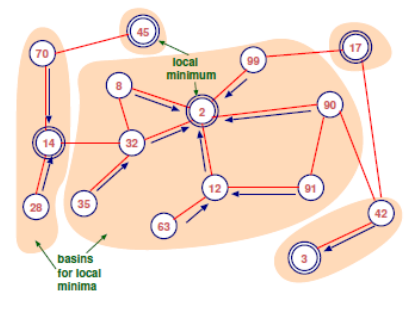
\includegraphics{images/LMS.png}}
\caption{Vyhledání objektu pro 1--hop okolí (okolí jednoho souseda).}
\label{LMS_search}
\end{center}
\end{figure}
%---konec obrazek
\begin{itemize}
\item Dotazování náhodně vyhledaných lokálních minim a zjišťování, zda obsahují požadovanou kopii objektu -- zpráva $search()$.
\item Příklad na obrázku \ref{LMS_search}. Číslo v uzlu je identifikátor a značí, jak daleko jsem k určitému typu objektu (tj. jak moc se ten identifikátor v uzlu liší od identifikátoru informace, kterou vyhledávám).
\begin{itemize}
\item Vybereme uzel (např. ten s hodnotou 91) -- kouknu se na svoje sousedy (dle velikosti sousedství -- $x$--hop neighborhoods, v tomto příkladě 1) a vyberu uzel s menším identifikátorem a přesunu se do něj (resp, dotaz pošlu pak skrze tento uzel) -- u nás uzel 12.
\item Opakujeme stále předchozí krok, dokud nenajdeme lokální minimum -- u nás hned v dalším kroku je to uzel s hodnotou 2 (protože je označený jako lokální minimum -- asi nějaký flag nebo něco takového, na přednášce jen řekl, že je to lokální minimum). Pokud nenajdu lokální minimum, tak musím přejít do jiného seskupení uzlů (oblasti) a tam vyhledávat.
\end{itemize}
\end{itemize}

\subsubsection*{Vzdálenost sousedů -- hop okolí}
%---obrazek
\begin{figure}[ht!]
\begin{center}
\scalebox{1.0}{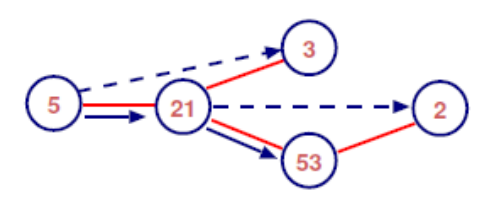
\includegraphics{images/hop.png}}
\caption{Hop okolí.}
\label{hop}
\end{center}
\end{figure}
%---konec obrazek
\begin{itemize}
\item Pokud budeme uvažovat třeba 2--hop okolí (vycházím z obrázku \ref{hop}) uzlu s hodnotou 5, tak 2--hop okolí budou uzly s hodnotami 21, 3 a 53. Z 21 pak 3, 53, 2.
\end{itemize}

\subsubsection{Shrnutí způsobů směrování}
\begin{itemize}
\item Flooding -- jednoduchá implementace, minimální paměťové a výpočetní nároky, neefektivní, špatně rozšiřitelná.
\item Náhodný průchod -- hledání čiště náhodné (bez znalosti umístění objektů), nalezení může trvat dlouho (v nejhorším případě se musí projít celá overlay).
\item LMS -- přidává znalosti (metrika vzdálenosti k objektu), směrování dle jména objektu (režie při hledání lokálních minim).
\end{itemize}

\subsection{Strukturované sítě}
\begin{itemize}
\item Kombinace geometrické struktury (uzel minimálně ví, že když pošle dotaz určitým směrem, tak to je blíž, a když ho pošle jiným směrem, tak je to dál -- je si vědom geometrické struktury -- rozdíl oproti nestrukturovaným) a směrování.
\item Distribuované směrovací algoritmy pomocí vzdálenosti (shoda prefixu, euklidovská či lineární vzdálenost, XOR) -- velikost směrovací tabulky ovlivněna počtem uzlů.
\end{itemize}

\subsubsection{Síť Pastry}
\begin{itemize}
\item Decentralizovaná, rozšiřitelná a samoorganizující se síť.
\item Je to framework pro určité P2P sítě (není konkrétní síť, co dělá konkrétní věci), které nad algoritmy pro Pastry můžu postavit. 
\item Pro sdílení souborů (systém PAST)$\ldots$
\item Složitost vyhledání je $O(log(N))$, kde $N$ je počet uzlů sítě (základ logaritmu závisí na tom, v jaké soustavě zapisujeme identifikátor -- dvojková 2 atp.).
\item Jmenný prostor $I$ tvoří: prostor identifikátorů uzlů (NodeID) -- např. hash IP adresy, tohle dostane uzel při přihlášení a prostor objektů (klíčů) -- podle tohoto jsou vyhledávány objekty.
\item Používají se 128--bitové identifikátory.
\end{itemize}

\subsubsection{Uzel sítě Pastry}
Uzel obsahuje:
\begin{itemize}
\item Identifikáto uzlu (NodeId) -- generován při připojení uzlu.
\item Tabulku listů $L$ -- uzly, které jsou numericky nejblíže.
\item Směrovací tabulku $R$ -- pro hledání cesty.
\item Tabulku sousedů $M$ -- uzly, které jsou vzdálenostně nejblíže.
\end{itemize}

\end{document}

